\documentclass[12pt,a4paper]{report}
\usepackage[utf8]{inputenc}
\usepackage[T1]{fontenc}
\usepackage[french]{babel}
\usepackage[a4paper,margin=2.5cm]{geometry}
\usepackage{lmodern}
\usepackage{setspace}
\usepackage{microtype}
\usepackage{hyperref}
\usepackage{enumitem}
\usepackage{graphicx}
\usepackage{caption}
\usepackage{pdflscape}
\usepackage{longtable}
\usepackage{array}
\usepackage{xcolor}
\hypersetup{colorlinks=true,linkcolor=black,urlcolor=blue,pdftitle={Rapport de projet — Plateforme Fitness}}
\onehalfspacing
\setcounter{tocdepth}{2}
\setlength{\LTpre}{0.5em}
\setlength{\LTpost}{0.5em}
\setlength{\tabcolsep}{2pt}

\makeatletter
\newcommand{\PlanStart}{%
  \vspace{0.8cm}
  \noindent\rule{\textwidth}{0.5pt}
  \vspace{0.6cm}
  \begin{center}\Large\bfseries Plan\end{center}
  \vspace{0.45cm}
}
\newcommand{\ChapterPlanStart}[1]{%
  \clearpage
  \refstepcounter{chapter}%
  \chaptermark{#1}%
  \addcontentsline{toc}{chapter}{\protect\numberline{\thechapter}#1}%
  \thispagestyle{plain}%
  \begin{center}
    {\large Chapitre~\thechapter\par}
    \vspace{0.8cm}
    {\Large\bfseries #1\par}
  \end{center}
  \vspace{0.6cm}
  \noindent\rule{\textwidth}{0.5pt}
  \vspace{0.6cm}
  \begin{center}\Large\bfseries Plan\end{center}
  \vspace{0.45cm}
}
\newcommand{\PlanEntry}[3]{%
  \@dottedtocline{1}{#2}{#3}{\hyperref[#1]{\ref*{#1}\hspace{0.65em}\nameref*{#1}}}{\hyperref[#1]{\pageref*{#1}}}
}
\newcommand{\PlanStarred}[1]{%
  \@dottedtocline{1}{0em}{3em}{\hyperref[#1]{\nameref*{#1}}}{\hyperref[#1]{\pageref*{#1}}}
}
\newcommand{\PlanSubEntry}[1]{%
  \@dottedtocline{2}{1.8em}{3.2em}{\hyperref[#1]{\ref*{#1}\hspace{0.65em}\nameref*{#1}}}{\hyperref[#1]{\pageref*{#1}}}
}
\newcommand{\ChapterBodyTitle}[1]{%
  \clearpage
  \begin{center}\large\bfseries Chapitre~\thechapter. #1\end{center}
  \vspace{0.5cm}
}
\makeatother

\begin{document}
\hypersetup{pageanchor=false}
\begin{titlepage}
  \centering
  \vspace*{2cm}
  {\Large Établissement : Tekup\\[0.4cm]}
  {\large filière : GLSI\\[2cm]}
  {\rule{\textwidth}{0.5pt}\\[0.6cm]}
  {\Huge\bfseries Rapport de projet\\[0.5cm]}
  {\LARGE Application de gestion et d’entraînement sportif\\[0.6cm]}
  {\rule{\textwidth}{0.5pt}\\[2cm]}
  \vfill
  \begin{flushleft}
    \textbf{Réalisé par :} Ahmed ikenjatoun\\
    \textbf{Année universitaire :} 2025--2026
  \end{flushleft}
\end{titlepage}

\hypersetup{pageanchor=true}
\pagenumbering{roman}
\chapter*{Résumé}
La plateforme Fitness étudiée dans ce rapport associe des fonctions de préparation et de suivi de l'entraînement à un catalogue de programmes et à une boutique. Le projet repose sur une interface web Next.js et React, une API NestJS et une base PostgreSQL manipulée avec Prisma. L'analyse du code distingue les parcours accessibles par l'API, les écrans de démonstration et les services métier qui ne sont pas encore raccordés à des routes. Le rapport présente le contexte, les besoins, l'architecture observée et les principaux domaines fonctionnels, puis précise les limites établies à partir du dépôt.

\noindent\textbf{Mots-clés :} entraînement sportif, application web, Next.js, NestJS, PostgreSQL, Prisma, UML.
\clearpage
\chapter*{Abstract}
This report studies a Fitness platform that combines workout planning and tracking with training programs and a product catalog. The project uses a Next.js and React web interface, a NestJS API, and PostgreSQL accessed through Prisma. The source review distinguishes API-backed user journeys from demonstration screens and service logic that is not yet connected to routes. The report describes the context, requirements, observed architecture, and main functional areas, while identifying limitations supported by the repository.

\noindent\textbf{Keywords:} fitness training, web application, Next.js, NestJS, PostgreSQL, Prisma, UML.
\clearpage
\tableofcontents
\clearpage
\listoffigures
\addcontentsline{toc}{chapter}{Liste des figures}
\clearpage
\listoftables
\addcontentsline{toc}{chapter}{Liste des tableaux}
\clearpage
\chapter*{Liste des abréviations}
\addcontentsline{toc}{chapter}{Liste des abréviations}
\begin{description}[leftmargin=2.8cm,style=nextline]
  \item[API] Application Programming Interface
  \item[DTO] Data Transfer Object
  \item[JWT] JSON Web Token
  \item[ORM] Object-Relational Mapping
  \item[PFE] Projet de fin d'études
  \item[RPE] Rate of Perceived Exertion
  \item[UML] Unified Modeling Language
\end{description}
\clearpage
\pagenumbering{arabic}

\chapter*{Introduction générale}
\addcontentsline{toc}{chapter}{Introduction générale}
Les applications numériques consacrées à l'activité physique regroupent aujourd'hui des fonctions de planification, de suivi et d'accompagnement. La plateforme étudiée réunit ces usages dans une application web et y associe des programmes sportifs ainsi qu'un espace de commerce. L'étendue de cette interface rend nécessaire une lecture précise des services effectivement disponibles : les pages visibles ne suffisent pas à établir qu'un parcours est persisté ou pris en charge par l'API.

Ce rapport s'appuie sur les fichiers présents dans le dépôt : application Next.js, API NestJS, schéma Prisma, contrôleurs, services, migrations et diagrammes. Il distingue les fonctionnalités reliées à des routes de celles qui sont seulement amorcées ou présentées par l'interface. Les informations d'entreprise, les résultats d'essais et le déroulement réel du projet ne figurant pas dans les sources, ils ne sont pas supposés.

Le premier chapitre situe le projet et expose la démarche de travail décrite dans le rapport. Le deuxième formalise les besoins, les acteurs, les diagrammes globaux et le découpage fonctionnel. La conclusion synthétise les constats et les suites à documenter.

\ChapterPlanStart{Cadre général du projet}
\PlanStarred{c1-intro}
\PlanEntry{c1-s1}{0em}{3.2em}
\PlanEntry{c1-s2}{0em}{3.2em}
\PlanSubEntry{c1-s2-sub1}
\PlanSubEntry{c1-s2-sub2}
\PlanSubEntry{c1-s2-sub3}
\PlanSubEntry{c1-s2-sub4}
\PlanSubEntry{c1-s2-sub5}
\PlanEntry{c1-s3}{0em}{3.2em}
\PlanSubEntry{c1-s3-sub1}
\PlanSubEntry{c1-s3-sub2}
\PlanStarred{c1-conclusion}
\clearpage
\ChapterBodyTitle{Cadre général du projet}
\phantomsection
\section*{Introduction}
\label{c1-intro}
\addcontentsline{toc}{section}{Introduction}
Ce chapitre situe la plateforme Fitness dans son contexte, précise le périmètre observé dans le dépôt et présente les choix d'organisation et de modélisation retenus. Les constats décrivent l'implémentation disponible au moment de l'analyse ; les informations institutionnelles absentes du dépôt sont signalées comme telles.

\section{Contexte général}
\label{c1-s1}
Les outils web et mobiles occupent une place croissante dans l'organisation de l'entraînement personnel. La conception examinée répond à un besoin de regroupement des fonctions de préparation des séances, de suivi des résultats et de consultation de contenus sportifs, avec un espace complémentaire de vente d'articles. Le dépôt matérialise ce périmètre au moyen d'une interface web, d'une API et d'une base relationnelle.

\section{Présentation du projet}
\label{c1-s2}
\subsection{Cadre général}
\label{c1-s2-sub1}
Le projet est une plateforme web Fitness destinée à des utilisateurs qui souhaitent créer des plans d'entraînement, enregistrer des séances et suivre leur activité. Le système comprend également des programmes structurés sur plusieurs semaines, un catalogue de produits, un panier et un service backend de recommandations adaptatives fondées sur les données de performance.

\subsection{Description du projet}
\label{c1-s2-sub2}
L'interface est réalisée avec Next.js 14, React et TypeScript. Le backend est une API REST modulaire construite avec NestJS. La persistance s'appuie sur PostgreSQL et Prisma. L'authentification utilise des jetons JWT et le hachage des mots de passe par bcrypt. Le client consomme l'API au moyen d'Axios ; Zustand conserve l'état d'authentification côté interface. Recharts est installé pour les visualisations, et Stripe figure dans les dépendances et dans le service de commande.

Le schéma Prisma comprend les comptes et les données de profil et d'abonnement, les exercices et séances, les programmes, les journaux de performance ainsi que les modèles du catalogue et des commandes. Le backend répartit ces domaines entre des modules NestJS dédiés. Les services accèdent directement à \texttt{PrismaService}; aucune couche repository distincte n'apparaît dans le dépôt.

\subsection{Étude de l'existant}
\label{c1-s2-sub3}
L'analyse porte sur les sources, les pages Next.js, les contrôleurs et services NestJS, le schéma Prisma, les migrations, les fichiers de configuration et la documentation fonctionnelle présente dans le dépôt. L'état observé associe des parcours utilisables à des interfaces de démonstration et à des fonctionnalités préparées côté service mais non raccordées à des routes.

Les parcours soutenus par des contrôleurs comprennent l'inscription et la connexion, la consultation des exercices et programmes, la gestion des plans et séances, l'inscription à un programme et le suivi de sa progression, les statistiques de séances, les fonctions du panier et le service adaptatif. À l'inverse, le contrôleur de commandes ne déclare aucune route, bien que son service contienne des opérations de création de commande et d'intention de paiement Stripe. La page calendrier emploie des dates d'exemple ; l'écran cartographique indique explicitement que l'intégration de carte reste à venir. Certaines visualisations analytiques utilisent également des séries codées en dur.

\subsection{Problématique}
\label{c1-s2-sub4}
La difficulté principale mise en évidence par l'examen est l'écart entre l'étendue fonctionnelle affichée par l'interface et les fonctions réellement persistées et exposées par l'API. Les écrans de profil et d'abonnement ne disposent pas d'opérations backend de mise à jour ou de facturation ; les commandes ne sont pas accessibles via leur contrôleur ; et les routes d'écriture des contenus sont protégées par JWT sans contrôle effectif du rôle administrateur. La documentation doit donc distinguer clairement l'existant opérationnel, les éléments partiels et les évolutions à réaliser.

\subsection{Solution proposée}
\label{c1-s2-sub5}
La solution présente une architecture séparant l'interface, les services métier et la persistance. L'API centralise les opérations sur les données d'entraînement, le catalogue et le panier. Le moteur d'adaptation analyse les journaux de performance à l'aide de règles déterministes explicables ; il ne s'agit pas d'un fournisseur d'intelligence artificielle externe. Pour compléter le périmètre présenté par l'interface, les évolutions prioritaires consistent à raccorder les fonctions inachevées et à renforcer le contrôle des droits avant leur mise à disposition.

\section{Présentation de la méthodologie de travail}
\label{c1-s3}
Dans le volet méthodologique, nous présentons le formalisme de modélisation retenu pour décrire la plateforme, puis le cadre de développement indiqué dans le rapport initial. Le dépôt ne contient pas de journal de sprints permettant de confirmer le déroulement effectif de cette méthode.

\subsection{Formalisme de modélisation}
\label{c1-s3-sub1}
    Pour la conception de notre plateforme Fitness, nous utilisons UML (Unified Modeling Language), un langage graphique de modélisation standard. UML complète les descriptions textuelles et facilite la compréhension de la structure du système ainsi que des interactions entre ses acteurs et ses fonctionnalités. Les diagrammes éditables du dépôt sont rédigés en PlantUML, qui transforme une description textuelle en diagramme \cite{plantuml}.

Les diagrammes UML utilisés dans notre rapport sont les suivants :
\begin{itemize}[leftmargin=*]
  \item Le diagramme de cas d'utilisation représente les principales fonctionnalités de la plateforme accessibles aux acteurs, notamment l'authentification, le suivi des entraînements, les programmes et les services de la boutique.
  \item Le diagramme de classes présente les principales entités métier de la plateforme et les associations qui les relient, telles que les utilisateurs, les exercices, les programmes et les séances.
\end{itemize}

Les diagrammes de cas d'utilisation et de classes présentés au chapitre suivant illustrent ces deux vues complémentaires.

\subsection{Méthodologie adoptée}
\label{c1-s3-sub2}
À mesure qu'un projet logiciel devient complexe et regroupe plusieurs fonctionnalités interdépendantes, une méthodologie est nécessaire pour organiser le travail et coordonner les activités de développement. Elle définit les règles de réalisation, les rôles et responsabilités, l'enchaînement des activités, l'organisation des tâches ainsi que les livrables attendus.

Parmi les méthodologies agiles les plus utilisées, nous pouvons citer XP (Extreme Programming), Kanban, FDD (Feature Driven Development) et SCRUM.

Le rapport initial indique Scrum comme cadre retenu. Le Guide Scrum décrit ce cadre comme une approche itérative et incrémentale organisée autour d'une équipe, d'événements, d'artefacts et de sprints \cite{scrum}. Il permet de répartir la réalisation en périodes courtes, de prioriser les exigences et de livrer progressivement des incréments fonctionnels. En l'absence de comptes rendus ou d'historique de projet, les releases et sprints décrits au chapitre suivant sont présentés comme une proposition de planification, non comme des itérations réalisées.

Ce cadre peut structurer une plateforme dont les fonctionnalités sont réparties entre plusieurs domaines, tels que l'entraînement, les programmes, le suivi des performances et la boutique. Il offre notamment les avantages suivants :
\begin{itemize}[leftmargin=*]
  \item une visibilité claire sur l'avancement du projet ;
  \item la possibilité de prioriser les fonctionnalités selon les besoins ;
  \item une adaptation aux changements des exigences ;
  \item le développement progressif des modules de la plateforme ;
  \item la division du projet en sprints facilement gérables ;
  \item la validation régulière des fonctionnalités développées.
\end{itemize}

\begin{figure}[htbp]
  \centering
  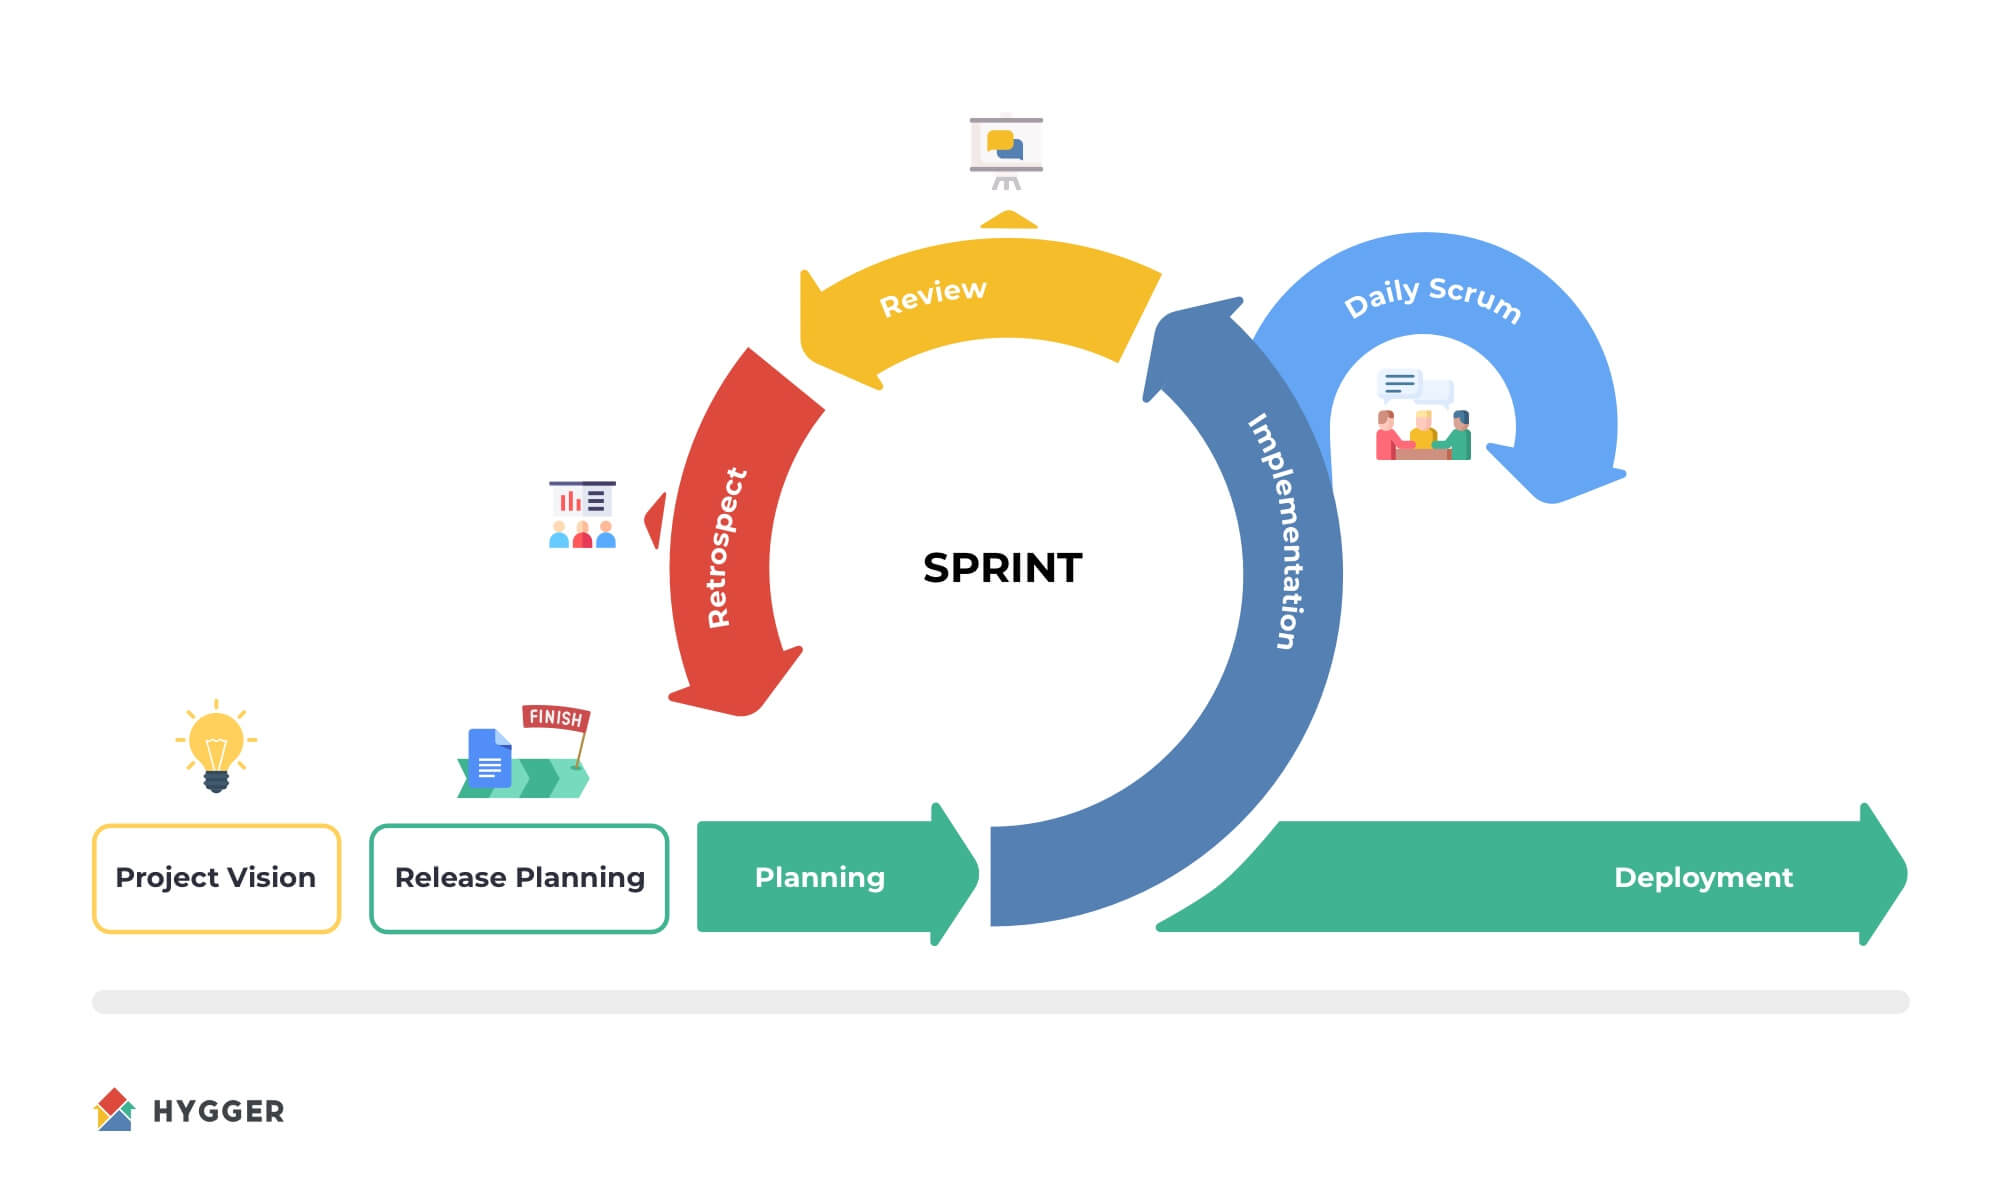
\includegraphics[width=0.97\textwidth,height=0.42\textheight,keepaspectratio]{docs/diagrams/scrum-cycle.jpg}
  \caption{Cycle de vie SCRUM}
  \label{fig:cycle-scrum}
\end{figure}

Le déroulement d'un sprint comprend les activités suivantes :
\begin{itemize}[leftmargin=*]
  \item \textbf{Sprint Planning :} l'équipe définit l'objectif du sprint et sélectionne les éléments prioritaires à réaliser.
  \item \textbf{Développement du sprint :} l'équipe conçoit, développe et vérifie les fonctionnalités retenues pendant la durée du sprint.
  \item \textbf{Daily Scrum :} un point quotidien permet de partager l'avancement et de coordonner le travail restant.
  \item \textbf{Sprint Review :} à la fin du sprint, l'équipe présente les fonctionnalités terminées et recueille les observations sur l'incrément produit.
  \item \textbf{Sprint Retrospective :} l'équipe examine le déroulement du sprint et identifie des améliorations à appliquer aux cycles suivants.
\end{itemize}

À l'issue du sprint, le \textbf{Product Increment} regroupe les fonctionnalités réalisées et intégrées. Il peut constituer une version potentiellement livrable de notre plateforme. La rétrospective permet à l'équipe d'améliorer progressivement son organisation et sa manière de travailler. Le chapitre suivant présente les besoins, les diagrammes globaux, puis le backlog, les releases et la planification des sprints de notre projet.

\phantomsection
\section*{Conclusion}
\label{c1-conclusion}
\addcontentsline{toc}{section}{Conclusion}
Ce chapitre a présenté le cadre logiciel, les technologies et les principaux écarts constatés entre les interfaces et les services disponibles. Cette distinction fonde l'analyse des besoins et la planification de compléments réalistes au chapitre suivant.

\ChapterPlanStart{Analyse et spécification des besoins}
\PlanStarred{c2-intro}
\PlanEntry{c2-s1}{0em}{3.2em}
\PlanSubEntry{c2-s1-sub1}
\PlanSubEntry{c2-s1-sub2}
\PlanSubEntry{c2-s1-sub3}
\PlanEntry{c2-s2}{0em}{3.2em}
\PlanEntry{c2-s3}{0em}{3.2em}
\PlanEntry{c2-s4}{0em}{3.2em}
\PlanSubEntry{c2-s4-sub1}
\PlanSubEntry{c2-s4-sub2}
\PlanSubEntry{c2-s4-sub3}
\PlanStarred{c2-conclusion}
\clearpage
\ChapterBodyTitle{Analyse et spécification des besoins}
\phantomsection
\section*{Introduction}
\label{c2-intro}
\addcontentsline{toc}{section}{Introduction}
Ce chapitre formalise les acteurs et les exigences de la plateforme, puis présente les diagrammes UML et le découpage fonctionnel. Les besoins sont qualifiés selon leur état dans le dépôt : implémenté par une route/service, partiel ou uniquement représenté par l'interface, ou à compléter.

\section{Spécification des besoins}
\label{c2-s1}
\subsection{Identification des acteurs}
\label{c2-s1-sub1}
\begin{singlespace}
\begin{longtable}{|p{4cm}|p{11.5cm}|}
\caption{Acteurs de la plateforme et périmètre associé}\label{tab:acteurs}\\
\hline
\textbf{Acteur} & \textbf{Rôle dans le périmètre observé} \\\hline
\endfirsthead
\hline
\textbf{Acteur} & \textbf{Rôle dans le périmètre observé} \\\hline
\endhead
Visiteur & Crée un compte, se connecte et consulte les contenus publics de programmes et de produits. \\\hline
Utilisateur authentifié & Gère ses plans et séances, suit des programmes, consulte ses statistiques, utilise le panier et les fonctions de suivi adaptatif. \\\hline
Administrateur & Rôle prévu par l'attribut \texttt{User.role} et par l'interface d'administration. Le backend ne vérifie pas actuellement ce rôle dans les opérations d'écriture ; cet acteur représente donc une responsabilité cible plutôt qu'une autorisation correctement appliquée. \\\hline
Moteur adaptatif & Composant interne qui calcule des indicateurs et recommandations à partir des performances. Il est fondé sur des règles déterministes et ne constitue pas un système externe d'IA. \\\hline
\end{longtable}
\end{singlespace}
\noindent Stripe est un système externe de paiement, et non un acteur de la plateforme. Le service contient une logique d'intention de paiement, mais le contrôleur de commandes ne l'expose pas.\par

\clearpage

\subsection{Besoins fonctionnels par acteur}
\label{c2-s1-sub2}
Les besoins fonctionnels de l'application sont définis selon les différents acteurs et les fonctionnalités attendues. L'état constaté correspond à l'état actuel de leur implémentation dans le projet.

\subsubsection{Visiteur}
Le visiteur doit pouvoir :
\begin{itemize}
    \item S'inscrire et s'authentifier.
    \item Parcourir les programmes d'entraînement et le catalogue public des produits.
\end{itemize}
\textbf{État constaté :} Les routes d'authentification, des programmes et des produits sont présentes.

\subsubsection{Utilisateur}

L'utilisateur doit pouvoir :
\begin{itemize}
    \item Consulter son identité et gérer son profil.
    \item Créer et gérer ses plans d'entraînement.
    \item Démarrer, terminer ou annuler une séance et consulter son historique.
\end{itemize}
\textbf{État constaté :} Les routes protégées sont présentes. La modification du profil est absente.

L'utilisateur doit également pouvoir :
\begin{itemize}
    \item Suivre un programme d'entraînement.
    \item Consulter son inscription et mettre à jour l'avancement des séances du programme.
\end{itemize}
\textbf{État constaté :} Les routes correspondantes sont présentes et le contrôle par JWT est utilisé.

Par ailleurs, l'utilisateur doit pouvoir :
\begin{itemize}
    \item Consulter ses statistiques.
    \item Enregistrer ses performances.
    \item Obtenir des recommandations adaptatives.
\end{itemize}
\textbf{État constaté :} Les statistiques de base et le service adaptatif sont présents. Certaines pages affichent toutefois des données d'exemple.

Concernant la marketplace, l'utilisateur doit pouvoir :
\begin{itemize}
    \item Parcourir les produits.
    \item Ajouter des articles au panier.
    \item Modifier les quantités et vider le panier.
\end{itemize}
\textbf{État constaté :} Le catalogue et les routes du panier sont présents.

Enfin, l'utilisateur doit pouvoir :
\begin{itemize}
    \item Planifier ses séances dans le calendrier.
    \item Gérer son abonnement.
    \item Effectuer une commande payée.
\end{itemize}
\textbf{État constaté :} L'interface et le calendrier sont partiels. Il n'existe pas d'API de programmation ou d'abonnement, et le contrôleur des commandes est vide.

\subsubsection{Administrateur}

L'administrateur doit pouvoir :
\begin{itemize}
    \item Gérer les utilisateurs.
    \item Gérer les exercices et les programmes.
    \item Gérer les produits et les commandes.
\end{itemize}
\textbf{État constaté :} Les opérations CRUD de certains contenus sont disponibles derrière une authentification JWT. Cependant, la gestion des utilisateurs est absente, aucun contrôle de rôle n'est implémenté et les commandes ne disposent pas de routes dédiées.


\subsection{Besoins non fonctionnels}
\label{c2-s1-sub3}
\begin{itemize}[leftmargin=*]
  \item \textbf{Sécurité :} authentification JWT, mots de passe hachés avec bcrypt, validation globale des entrées via \texttt{ValidationPipe}. Le contrôle de rôle administrateur et les routes d'abonnement/commande restent à compléter.
  \item \textbf{Intégrité :} PostgreSQL et contraintes/relations assurent la persistance relationnelle ; les DTO valident les données des routes concernées.
  \item \textbf{Maintenabilité :} modules NestJS séparés par domaine, composants et pages Next.js, types TypeScript et schéma centralisé.
  \item \textbf{Interopérabilité :} échanges entre frontend et backend par API REST ; la configuration CORS observée autorise actuellement l'origine de développement.
  \item \textbf{Ergonomie et adaptation :} interface web responsive visée ; l'expérience doit distinguer les données réellement disponibles des éléments de démonstration.
  \item \textbf{Confidentialité :} les données d'entraînement étant rattachées aux utilisateurs, les opérations doivent rester limitées au propriétaire ; les contrôles d'accès doivent être vérifiés pour chaque ressource.
\end{itemize}

\section{Diagramme de cas d'utilisation global}
\label{c2-s2}
Le diagramme de cas d'utilisation global présente les principaux parcours fonctionnels visés pour l'application Fitness, du point de vue des utilisateurs et de l'administrateur. Il inclut les services externes représentés dans la vue fonctionnelle. Cette figure exprime le périmètre fonctionnel attendu ; elle ne signifie pas que chaque parcours est déjà exposé par une route backend. L'état d'implémentation et les limites relevées dans le dépôt sont décrits dans les sections correspondantes. La figure~\ref{fig:cas-utilisation-global} complète l'état détaillé des besoins du tableau~\ref{tab:besoins-fonctionnels}.

\clearpage
\begin{landscape}
\begin{figure}[p]
  \centering
  \makebox[\textwidth][c]{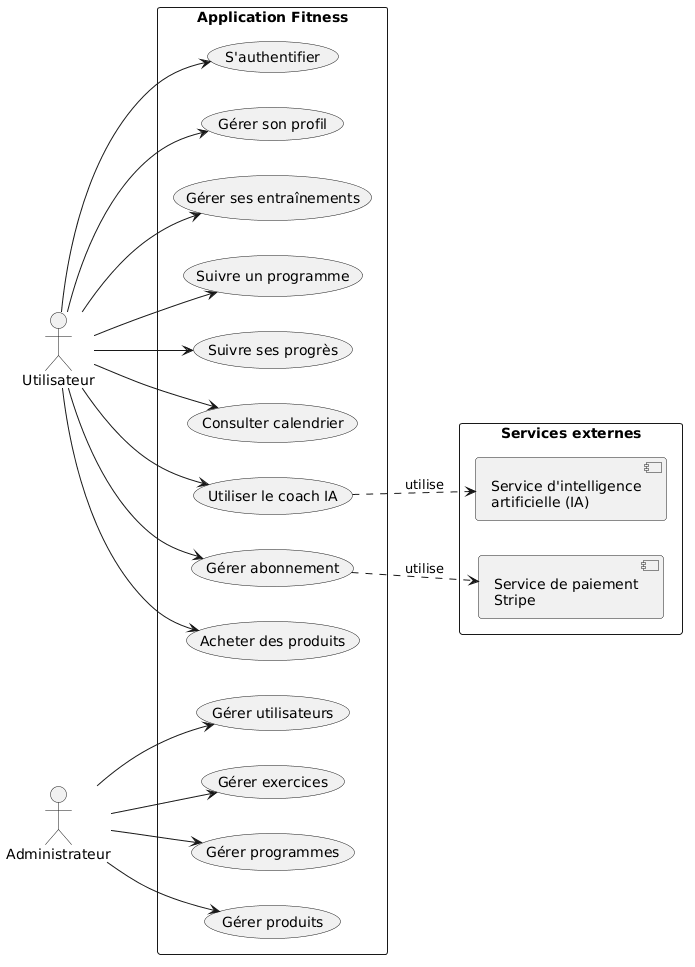
\includegraphics[width=0.85\paperheight,height=0.65\paperwidth,keepaspectratio]{docs/diagrams/cas-utilisation.png}}
  \caption{Diagramme de cas d'utilisation — périmètre étayé par le dépôt}
  \label{fig:cas-utilisation-global}
\end{figure}
\end{landscape}
\clearpage

\section{Diagramme de classes global}
\label{c2-s3}
Le diagramme de classes global présente une vue métier d'ensemble des utilisateurs, programmes, séances, performances, abonnements, paiements et produits. Il rassemble les classes et relations de la conception fonctionnelle illustrée par la figure~\ref{fig:classes-global} ; il ne constitue pas une transcription du schéma Prisma. Les différences entre ce modèle métier et la persistance réellement déclarée sont précisées ci-dessous.

\clearpage
\begin{landscape}
\begin{figure}[p]
  \centering
  \makebox[\textwidth][c]{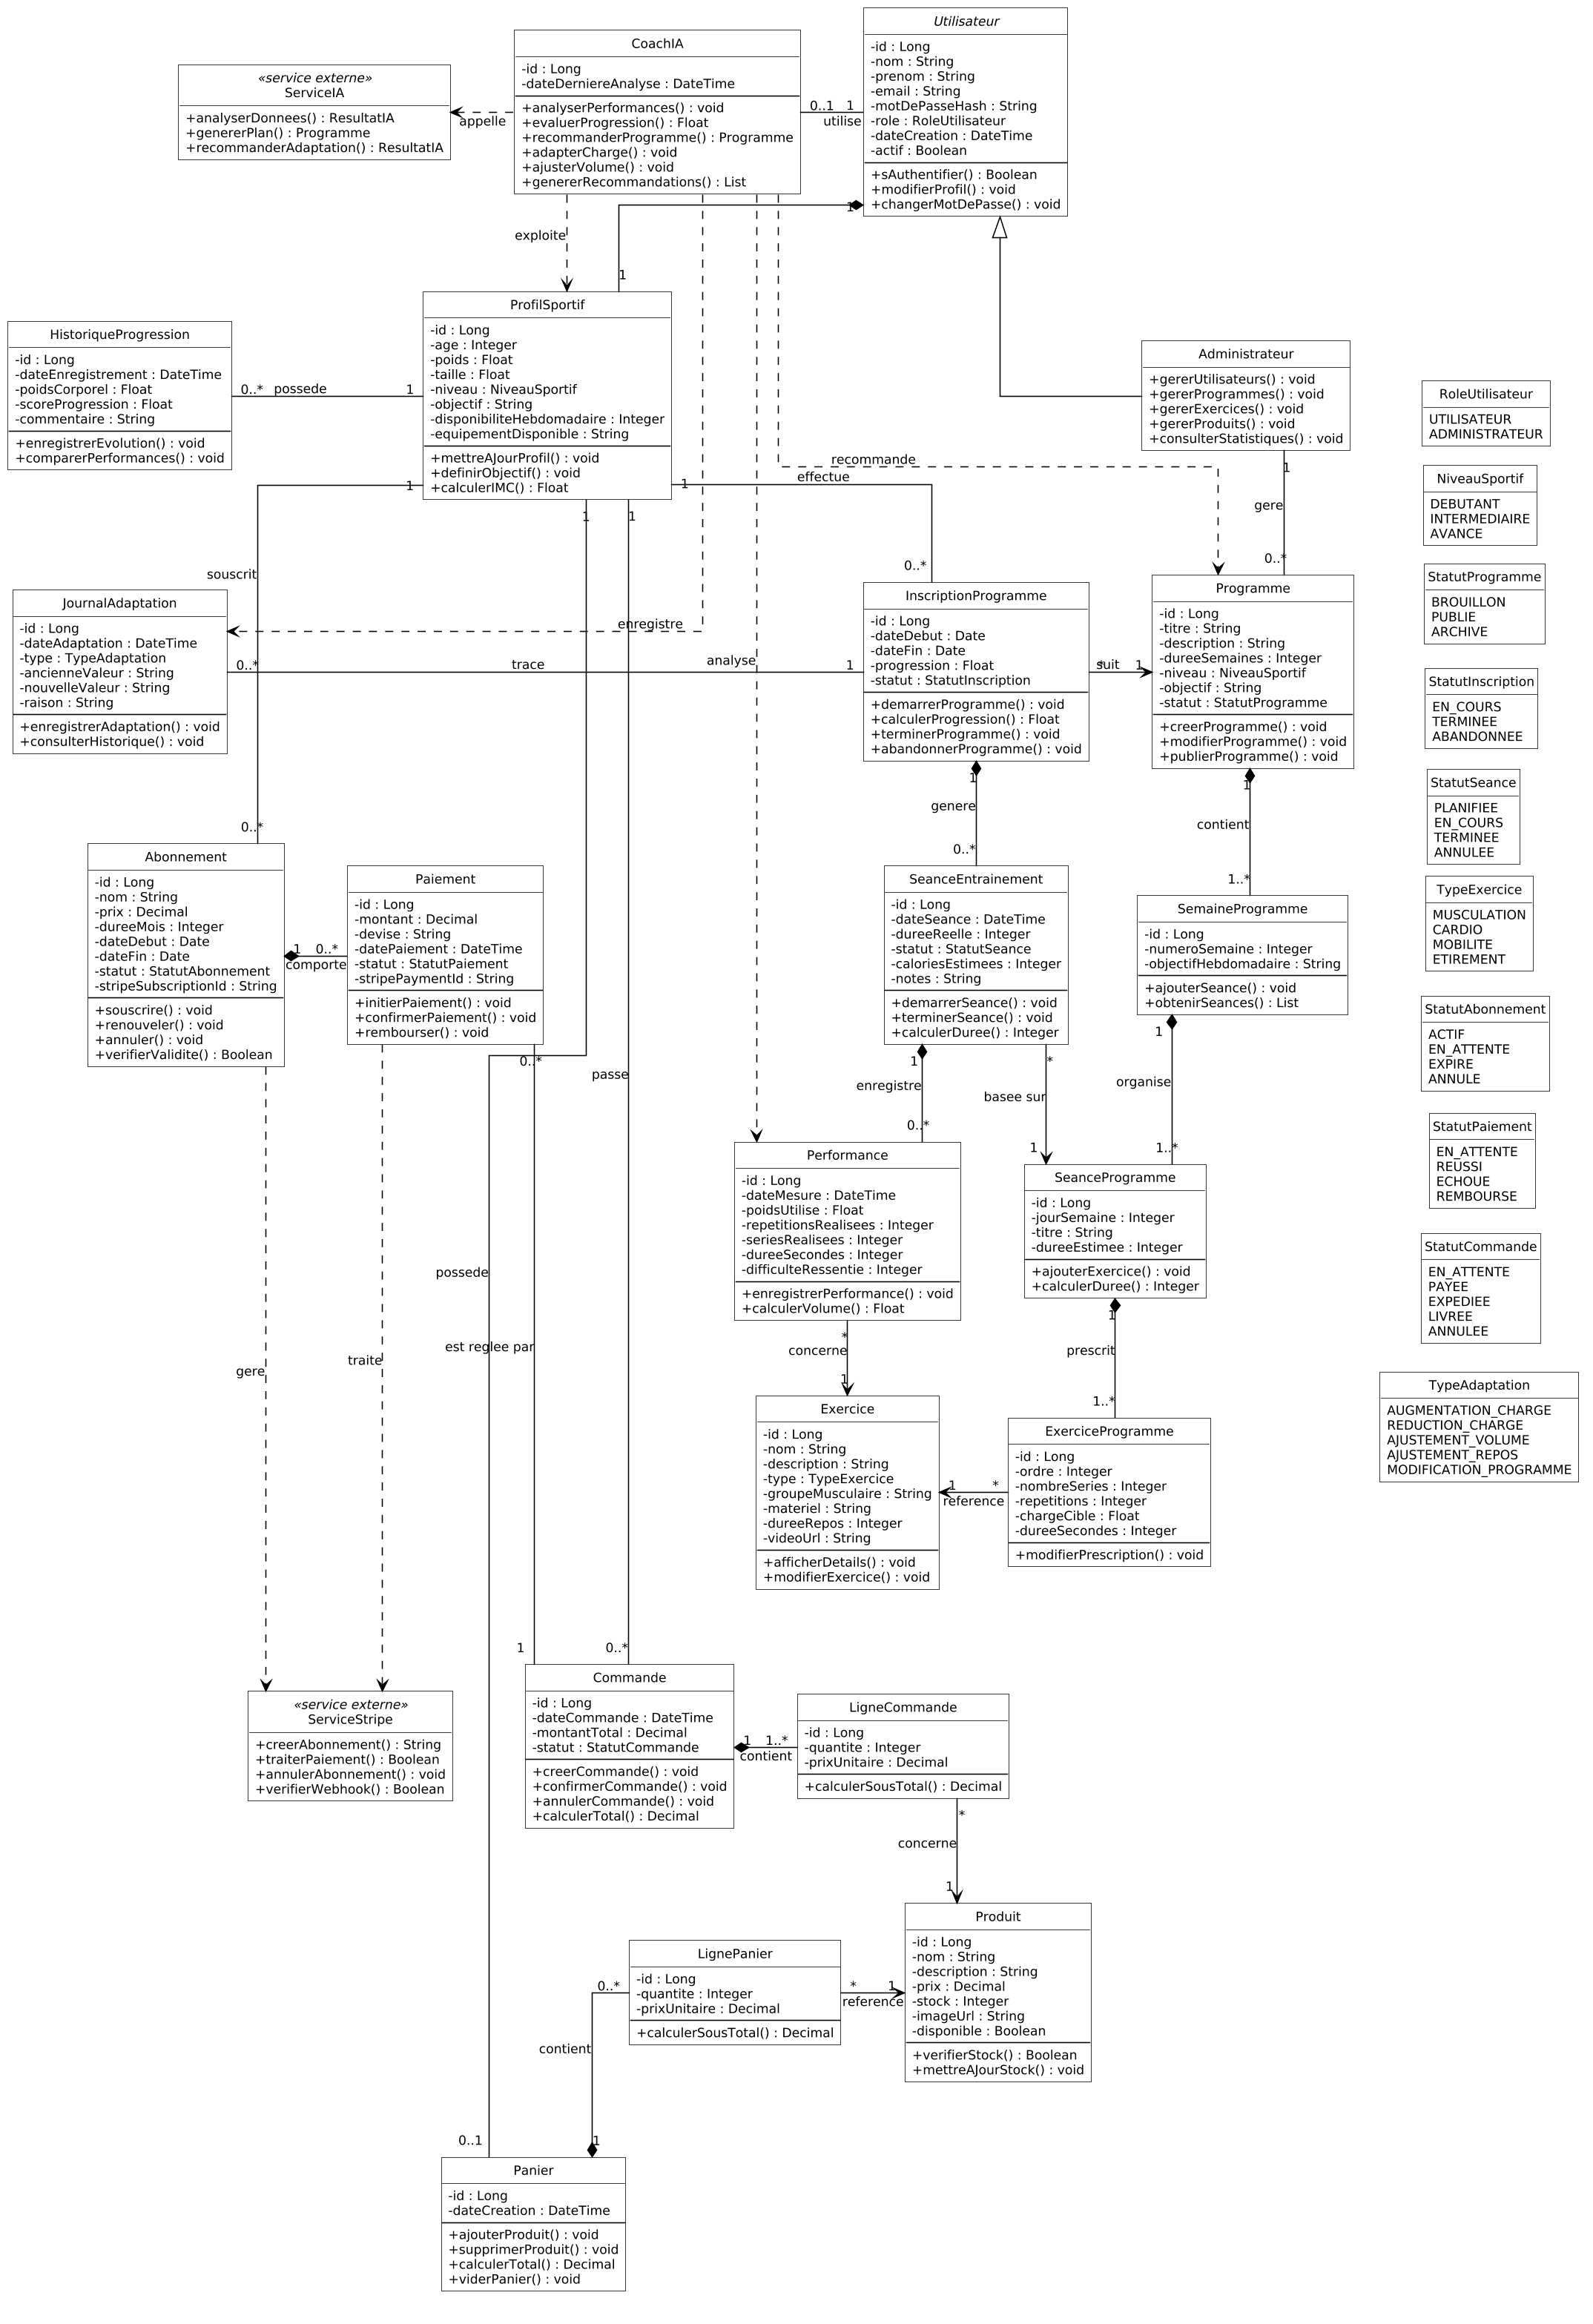
\includegraphics[width=0.94\paperheight,height=0.74\paperwidth,keepaspectratio]{docs/diagrams/classes-global.png}}
  \caption{Diagramme de classes global — principaux modèles Prisma de la plateforme}
  \label{fig:classes-global}
\end{figure}
\end{landscape}
\clearpage

Dans l'implémentation Prisma, les informations de profil et d'abonnement (taille, poids, objectif, formule et état) sont portées par \texttt{User}; les modèles distincts \texttt{ProfilSportif} et \texttt{Abonnement} du diagramme n'existent pas. Les données de paiement sont portées par \texttt{Order}, sans modèle \texttt{Paiement} séparé. L'adaptation est journalisée par \texttt{AdaptationLog}; le coaching est assuré par une logique backend et aucun modèle \texttt{CoachIA} ni service externe d'IA n'est déclaré. Les modèles de commande et de paiement ne disposent pas non plus de routes backend exposées à ce jour.

\section{Structure et découpage du projet}
\label{c2-s4}
Le découpage fonctionnel suit les modules présents dans l'API et les espaces de l'interface : authentification, utilisateurs, exercices, plans et séances, programmes, adaptation, catalogue, panier et commandes. Les priorités ci-dessous combinent l'état observé et l'ordre proposé pour terminer les parcours. Les durées sont des estimations indicatives en jours ouvrés, et ne proviennent pas d'un outil de suivi de projet.

\subsection{Product Backlog global}
\label{c2-s4-sub1}
\footnotesize
\begin{singlespace}
\begin{longtable}{|p{1cm}|p{4cm}|p{0.9cm}|p{7cm}|p{1.4cm}|p{1.35cm}|}
\caption{Backlog produit proposé à partir des besoins et des écarts observés}\label{tab:product-backlog}\\
\hline
\textbf{ID} & \textbf{Fonctionnalité} & \textbf{ID} & \textbf{User Story} & \textbf{Priorité} & \textbf{Durée} \\\hline
\endfirsthead
\hline
\textbf{ID} & \textbf{Fonctionnalité} & \textbf{ID} & \textbf{User Story} & \textbf{Priorité} & \textbf{Durée} \\\hline
\endhead
F01 & Authentification et profil & PB01 & En tant que visiteur, je veux créer un compte et me connecter afin d'accéder à mon espace. & P1 & 2 j \\\hline
F01 & Authentification et profil & PB02 & En tant qu'utilisateur, je veux consulter mes informations de compte et mettre à jour mon profil. & P1 & 1,5 j \\\hline
F02 & Exercices et entraînements & PB03 & En tant qu'utilisateur, je veux consulter et gérer les exercices proposés. & P1 & 2,5 j \\\hline
F02 & Exercices et entraînements & PB04 & En tant qu'utilisateur, je veux créer et gérer mes plans d'entraînement. & P1 & 2,5 j \\\hline
F02 & Exercices et entraînements & PB05 & En tant qu'utilisateur, je veux démarrer, terminer, annuler et retrouver mes séances. & P1 & 2,5 j \\\hline
F02 & Exercices et entraînements & PB06 & En tant qu'utilisateur, je veux enregistrer mes séries, charges, répétitions et RPE. & P1 & 2,5 j \\\hline
F02 & Exercices et entraînements & PB07 & En tant qu'utilisateur, je veux consulter mes statistiques issues de mes séances. & P1 & 1,5 j \\\hline
F03 & Programmes sportifs & PB08 & En tant qu'utilisateur, je veux parcourir des programmes et consulter leur contenu. & P1 & 1,5 j \\\hline
F03 & Programmes sportifs & PB09 & En tant qu'utilisateur, je veux m'inscrire à un programme et suivre son avancement. & P1 & 2,5 j \\\hline
F04 & Coaching adaptatif & PB10 & En tant qu'utilisateur, je veux obtenir des conseils adaptés à mes performances récentes. & P2 & 4 j \\\hline
F05 & Calendrier sportif & PB11 & En tant qu'utilisateur, je veux consulter et planifier mon calendrier d'entraînement. & P2 & 2,5 j \\\hline
F06 & Boutique et commandes & PB12 & En tant qu'utilisateur, je veux consulter les produits et leurs détails. & P2 & 1,5 j \\\hline
F06 & Boutique et commandes & PB13 & En tant qu'utilisateur, je veux ajouter, modifier et retirer des articles de mon panier. & P2 & 2,5 j \\\hline
F06 & Boutique et commandes & PB14 & En tant qu'utilisateur, je veux créer une commande et payer avec Stripe. & P2 & 4 j \\\hline
F06 & Boutique et commandes & PB15 & En tant qu'utilisateur, je veux consulter mes commandes et leur état. & P2 & 2,5 j \\\hline
F07 & Abonnements & PB16 & En tant qu'abonné, je veux choisir, payer et gérer une formule Free, Pro ou Elite. & P2 & 4 j \\\hline
F08 & Administration & PB17 & En tant qu'administrateur, je veux administrer les produits, programmes et exercices avec des droits vérifiés. & P1 & 4 j \\\hline
F08 & Administration & PB18 & En tant qu'administrateur, je veux gérer les utilisateurs et les commandes. & P3 & 4 j \\\hline
F09 & Activités extérieures & PB19 & En tant qu'utilisateur pratiquant une activité extérieure, je veux visualiser mes parcours sur une carte. & P3 & 4 j \\\hline
\end{longtable}
\end{singlespace}
\normalsize

P1 désigne une priorité haute pour la cohérence et la sécurité du socle ; P2 désigne une capacité importante à compléter après le socle ; P3 correspond à une évolution secondaire. Les durées estimées couvrent l'analyse, l'implémentation et la validation d'une user story dans un contexte d'équipe ; elles devront être réévaluées selon les critères d'acceptation et la vélocité réels.

\subsection{Planification des releases}
\label{c2-s4-sub2}
\begin{singlespace}
\begin{longtable}{|p{1.5cm}|p{3.9cm}|p{7cm}|p{4cm}|}
\caption{Planification indicative des releases}\label{tab:releases}\\
\hline
\textbf{Release} & \textbf{Objectif} & \textbf{Contenu proposé} & \textbf{État de référence} \\\hline
\endfirsthead
\hline
\textbf{Release} & \textbf{Objectif} & \textbf{Contenu proposé} & \textbf{État de référence} \\\hline
\endhead
R1 & Socle d'entraînement & Authentification, exercices, plans, séances, historique et statistiques réelles. & Majoritairement présent ; profil éditable à compléter. \\\hline
R2 & Programmes et adaptation & Catalogue des programmes, inscription, progression, journal de performance et conseils adaptatifs. & API et logique principales présentes ; raccordement UI à vérifier. \\\hline
R3 & Commerce & Catalogue, panier, création de commande, paiement Stripe, suivi de commande et administration sécurisée. & Catalogue et panier présents ; commande/paiement non exposés par API. \\\hline
R4 & Services complémentaires & Cycle d'abonnement, calendrier persistant, administration des comptes et carte d'activités. & Partiel ou absent selon fonctionnalité. \\\hline
\end{longtable}
\end{singlespace}
Ces releases constituent une proposition de livraison fondée sur l'état du code et ne correspondent pas à des versions déjà publiées documentées dans le dépôt.

\subsection{Planification des sprints}
\label{c2-s4-sub3}
\begin{singlespace}
\begin{longtable}{|p{1.5cm}|p{3cm}|p{9cm}|p{3cm}|}
\caption{Planification indicative des sprints}\label{tab:sprints}\\
\hline
\textbf{Sprint} & \textbf{But} & \textbf{Éléments proposés} & \textbf{Livrable} \\\hline
\endfirsthead
\hline
\textbf{Sprint} & \textbf{But} & \textbf{Éléments proposés} & \textbf{Livrable} \\\hline
\endhead
S1 & Fiabiliser le socle & Valider inscription/connexion, lecture du compte, CRUD des exercices et plans ; ajouter l'édition du profil et les tests d'accès par propriétaire. & R1 cohérente. \\\hline
S2 & Terminer le suivi sportif & Valider le cycle de vie des séances, compléter l'enregistrement des séries et remplacer les statistiques codées en dur par des données API. & Suivi basé sur données réelles. \\\hline
S3 & Consolider les programmes & Vérifier consultation, inscription et progression ; raccorder de manière fiable le panneau d'adaptation et distinguer la logique déterministe d'une IA externe. & R2 intégrée. \\\hline
S4 & Sécuriser et terminer le commerce & Ajouter contrôle de rôle, routes d'orders, paiement Stripe, traitement confirmé, consultation des commandes et gestion cohérente du stock. & Parcours d'achat complet. \\\hline
S5 & Compléter les services premium & Ajouter persistance et API du calendrier, cycle de facturation des abonnements et intégration cartographique si ces fonctions restent dans le périmètre. & R4 selon arbitrage. \\\hline
\end{longtable}
\end{singlespace}
L'ordre et les livrables sont une planification indicative déduite des lacunes ; aucune durée ni vélocité n'est inventée en l'absence de calendrier de projet et de données d'équipe.

\phantomsection
\section*{Conclusion}
\label{c2-conclusion}
\addcontentsline{toc}{section}{Conclusion}
L'analyse distingue les fonctions soutenues par l'API des interfaces de démonstration et des services non exposés. Les diagrammes décrivent le périmètre fonctionnel et un échantillon des entités réellement définies, tandis que le backlog traduit les écarts relevés en un ordre de réalisation cohérent. Cette base peut être enrichie par les informations institutionnelles et le suivi réel de l'équipe.

\chapter*{Conclusion générale et perspectives}
\addcontentsline{toc}{chapter}{Conclusion générale et perspectives}
Ce rapport a étudié une plateforme web de gestion de l'entraînement et de programmes sportifs, complétée par un espace de commerce. L'analyse du dépôt a permis de décrire son architecture Next.js, NestJS et PostgreSQL/Prisma, ainsi que les principaux modèles et parcours métier. Elle a également mis en évidence la nécessité de distinguer les pages de démonstration, les services présents et les opérations réellement exposées par l'API.

Les suites identifiées concernent le raccordement des parcours incomplets, la vérification des droits d'administration et la production d'éléments de validation reproductibles. Pour rendre le rapport pleinement représentatif d'un PFE, il reste à intégrer les informations institutionnelles et d'encadrement, la chronologie réelle du projet, les décisions méthodologiques effectivement suivies, les résultats des tests réalisés et, le cas échéant, les preuves de déploiement. Ces informations ne peuvent être établies à partir du dépôt seul.

\renewcommand{\bibname}{Webographie}
\begin{thebibliography}{9}
\addcontentsline{toc}{chapter}{Webographie}
\bibitem{nextjs} Vercel, \emph{Next.js Documentation}, \url{https://nextjs.org/docs}, consulté le 11 octobre 2026.
\bibitem{nestjs} NestJS, \emph{Documentation officielle}, \url{https://docs.nestjs.com/}, consulté le 11 octobre 2026.
\bibitem{prisma} Prisma, \emph{Upgrade to Prisma ORM v5}, \url{https://www.prisma.io/docs/guides/upgrade-prisma-orm/v5}, consulté le 11 octobre 2026.
\bibitem{postgres} PostgreSQL Global Development Group, \emph{PostgreSQL Documentation}, \url{https://www.postgresql.org/docs/current/}, consulté le 11 octobre 2026.
\bibitem{plantuml} PlantUML, \emph{Language Reference Guide}, \url{https://plantuml.com/}, consulté le 11 octobre 2026.
\bibitem{scrum} Ken Schwaber et Jeff Sutherland, \emph{The Scrum Guide}, novembre 2020, \url{https://scrumguides.org/scrum-guide.html}, consulté le 11 octobre 2026.
\end{thebibliography}
\end{document}

